\documentclass{article}
\usepackage[utf8]{inputenc}
\usepackage{bm}
\usepackage[bbgreekl]{mathbbol}

\usepackage{multicol}
\usepackage{graphicx}
\usepackage{epsfig}
\usepackage{lipsum}
\usepackage{amsmath}
\usepackage{amscd}
\usepackage{graphpap}
\usepackage{amssymb}
\usepackage{epstopdf}
\usepackage[dvipsnames]{xcolor}
\usepackage{cancel}
\usepackage[left=0.5in,right=0.5in,top=0.5in,bottom=0.5in]{geometry}
\DeclareGraphicsRule{.tif}{png}{.png}{`convert #1 `dirname #1`/`basename #1 .tif`.png}
%%%%%\usepackage{natbib}
\usepackage{epsf}
\epsfclipon
\pagestyle{plain}

\newcommand{\bF}{\mathbf{F}}
\newcommand{\bg}{\mathbf{g}}
\newcommand{\bn}{\mathbf{n}}
\newcommand{\bu}{\mathbf{u}}

\newcommand{\bbI}{\mathbb{I}}

\newcommand{\grad}{\nabla}
\newcommand{\Lap}{\nabla^2}
\newcommand{\parens}[1]{\mathopen{}\left(#1\right)\mathclose{}}

\begin{document}
\begin{center}
\Large \textbf{Running and visualizing the IBAMR tutorials}
\end{center}
\section{Navier Stokes Ex 1}
Open a terminal and log in to one of the clot servers.
\begin{verbatim}
ssh username@clot128a.math.utah.edu
\end{verbatim}
where \verb|username| is your math username. You will be asked to type your password. Create and navigate to a folder that you will use to build the IBAMR examples. Clone the github repository into that directory
\begin{verbatim}
mkdir ibamr_tutorials && cd ibamr_tutorials
git clone https://github.com/abarret/ibamr_tutorial.git
\end{verbatim}
At this point, you will have the IBAMR examples in a directory named \verb|ibamr_tutorial|. It contains the examples and CMake build system files. Next, we create a build directory and run \verb|CMake| to generate the Makefiles that can be used to compile the examples. This searches the provided directory for the IBAMR header files and compiled libraries.
\begin{verbatim}
mkdir build && cd build
cmake ../ibamr_tutorial -DIBAMR_ROOT=/u/ma/barrett/ibamr/ibamr/linux-opt \
  -DCMAKE_CXX_COMPILER=/u/ma/barrett/ibamr/openmpi/4.1.3/bin/mpicxx
\end{verbatim}
Note that this uses the same compiler flags that were used to build IBAMR, in this case those are \verb|-O3 -march=native|. Now we can build the examples.
\begin{verbatim}
make -j4 examples
\end{verbatim}
The argument \verb|-j4| will parallelize the build and compile at most 4 files at the same time. Once \verb|CMake| is run correctly, the Makefiles will automatically track changes in depedencies, and automatically determine which files need to be recompiled when running \verb|make|. Now you can navigate into one of the examples and run it.
\begin{verbatim}
cd navier_stokes-ex1
./main2d input2d
\end{verbatim}
This example is a simulation of the Kelvin-Helmholtz instability, in which the initial conditions consist of a sharp shear layer with a small perturbation. While this is running, we will open VisIt to visualize the results. At this time, you must use VisIt version 3.3 or 3.4. We will set up VisIt can be run in client-server mode to visualize results remotely. Alternatively, you can download the visualization files to analyze them locally.

With VisIt open in the \verb|Options| menu, click the \verb|Host profiles| button. Create a new host and set it as in the following image. If you are using a different minor version than 3.3, you should use the appropriate VisIt release. Minor versions for the client and the server must match. The path to the VisIt installation should be the path to the executable, without the \verb|bin/visit| extension.
\begin{center}
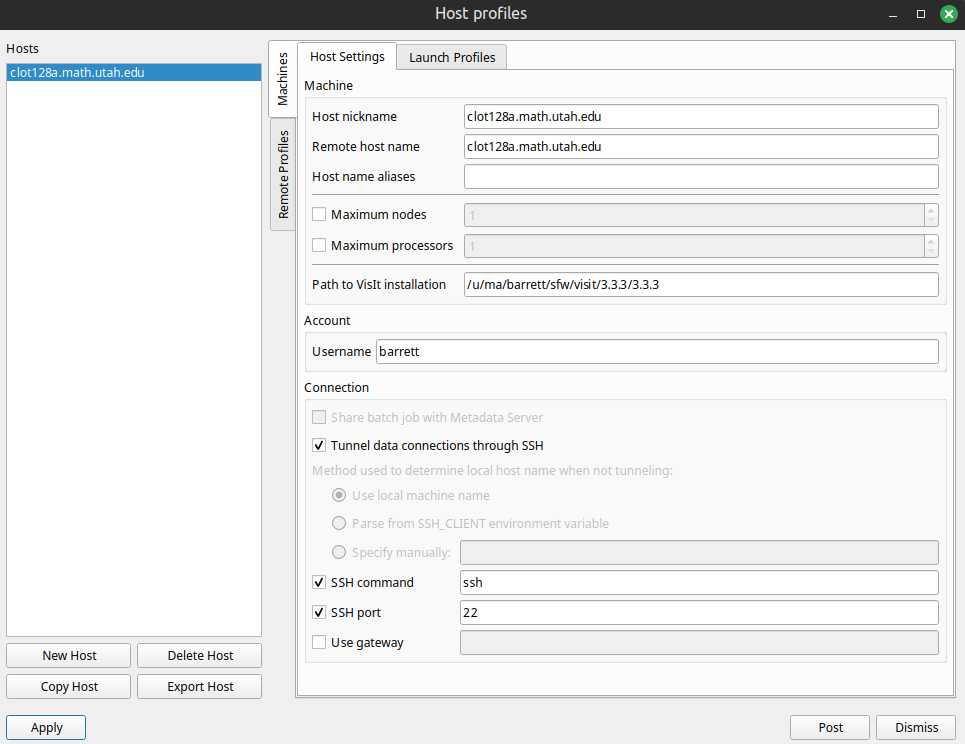
\includegraphics[width=0.75\textwidth]{Graphs/visit_host_profiles.png}
\end{center}
Click apply and dismiss. Now we can connect to the clot server. Click \verb|Open| and change the host to \verb|clot128a.math.utah.edu|. You will be asked for your password. Now navigate to the build directory and open the \verb|dumps.visit| file
\begin{center}
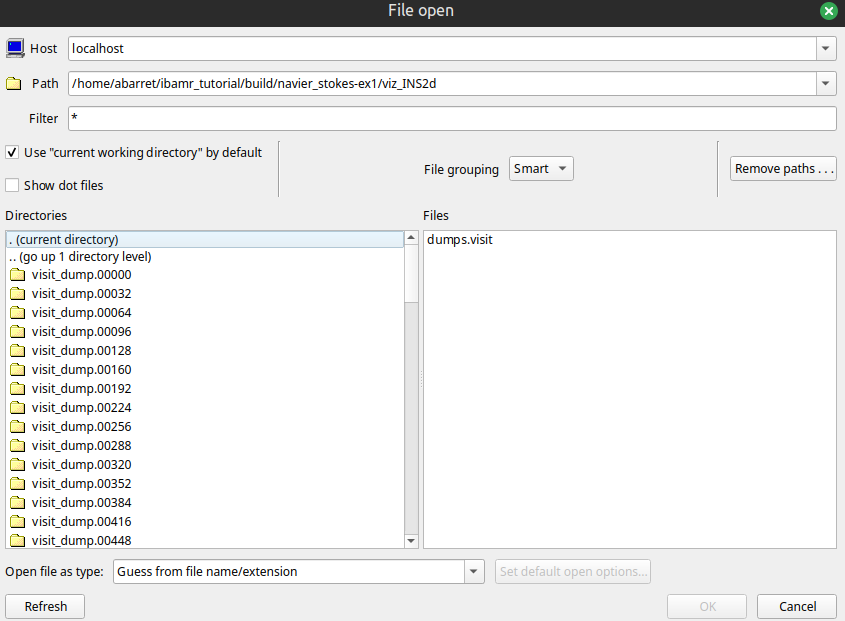
\includegraphics[width=0.75\textwidth]{Graphs/visit_ns-ex1.png}
\end{center}
By default, if running with multiple levels, a levels outline will be created by default. Now you can add various plots through the \verb|Add| button. In particular, we can add a color plot of the velocity magnitude by selecting \verb|Add|, then \verb|Pseudocolor|, then \verb|U_magnitude|.
\begin{center}
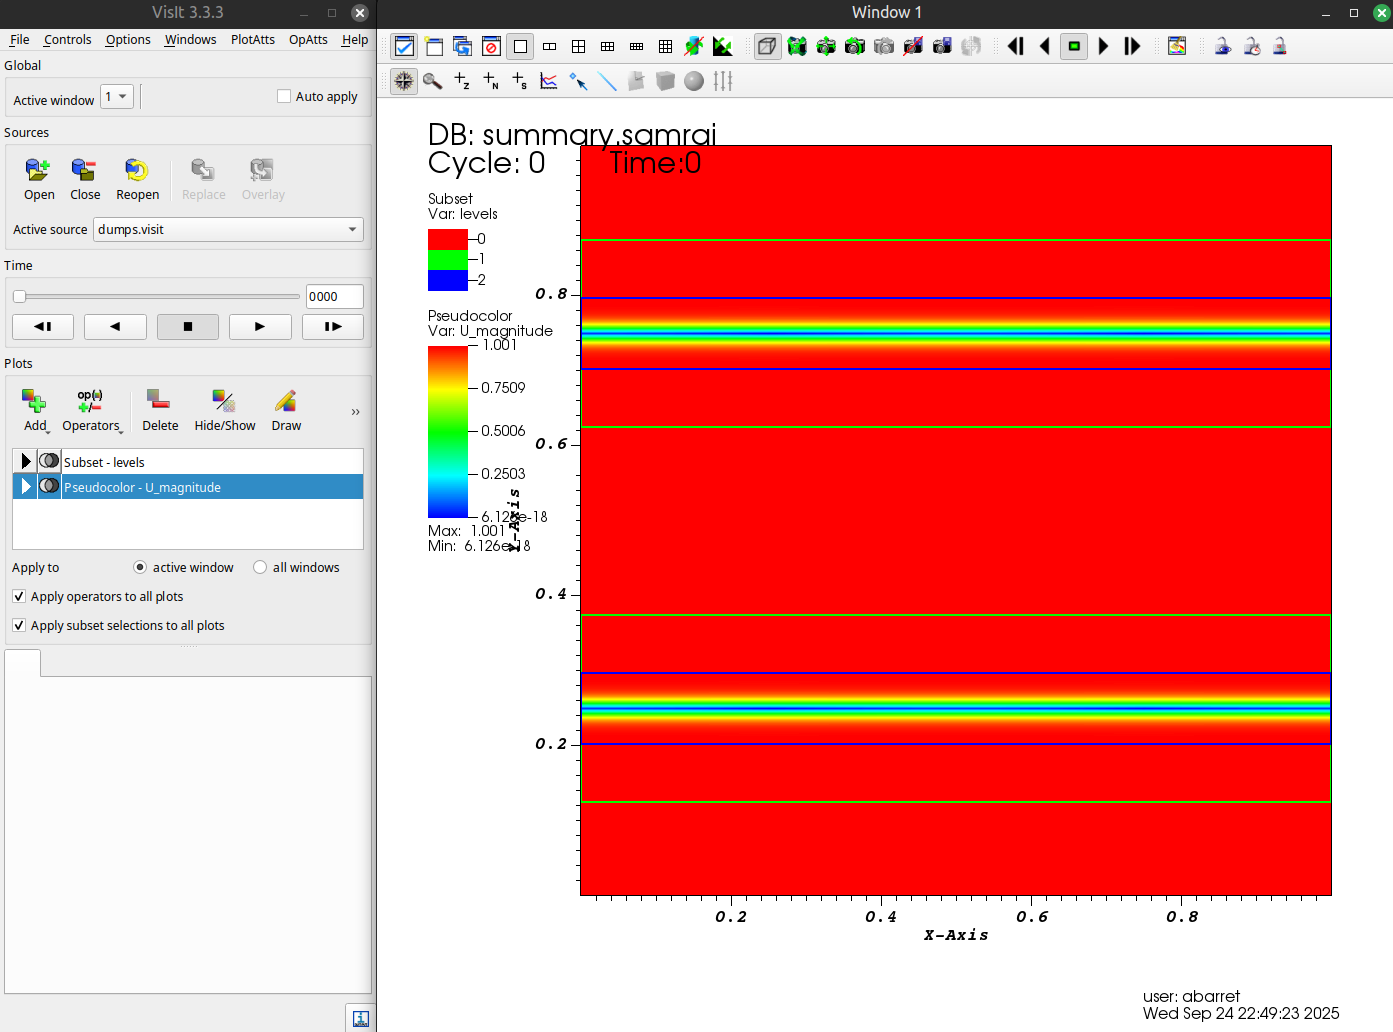
\includegraphics[width=0.75\textwidth]{Graphs/visit_u_mag.png}
\end{center}
Make sure to click \verb|Draw| after adding any plot that you want to visualize. Double click any of the plots in the list to look at different plotting options, setting, e.g. color bars, color tables, line widths, and more. You can animate over time by pressing to play button.

\section{IB Ex 1}
As before, we want to navigate to the build directory of the IBAMR tutorials.
\begin{verbatim}
cd ${HOME}/ibamr_tutorial/build
\end{verbatim}
For this example, we want to build \verb|IB-ex1|, which is the classic IB simulation of an elastic rubberband.
\begin{verbatim}
make IB-ex1 && cd IB-ex1
\end{verbatim}
Note that if \verb|make| determines that no depedencies have changed, then the tool may correctly not compile anything. In this directory, in addition to the compiled binary and input file, there are several \verb|.spring| and \verb|.vertex| files. These files set the initial configuration and elasticity of the immersed structure. There is also a MATLAB file \verb|generate_curve2d.m| that will generate these input files. Looking at the \verb|curve2d_64| files, they begin with
\begin{multicols}{2}
\begin{verbatim}
cat curve2d_64.vertex
304
6.7857142857142860e-01 5.0000000000000000e-01
6.7853328871213048e-01 5.0723341542964395e-01
6.7841888542630380e-01 5.1446374098708458e-01
6.7822826758319077e-01 5.2168788812000810e-01
6.7796151660833393e-01 5.2890277091531634e-01
6.7761874644879327e-01 5.3610530741732487e-01
6.7720010352447235e-01 5.4329242094427166e-01
6.7670576666557192e-01 5.5046104140257135e-01
6.7613594703620039e-01 5.5760810659825688e-01
6.7549088804417134e-01 5.6473056354504547e-01
6.7477086523702756e-01 5.7182536976847198e-01
\end{verbatim}
\columnbreak
\begin{verbatim}
cat curve2d_64.spring
304
 0      1 1.9353241079974475e+02 0.0000000000000000e+00
 1      2 1.9353241079974475e+02 0.0000000000000000e+00
 2      3 1.9353241079974475e+02 0.0000000000000000e+00
 3      4 1.9353241079974475e+02 0.0000000000000000e+00
 4      5 1.9353241079974475e+02 0.0000000000000000e+00
 5      6 1.9353241079974475e+02 0.0000000000000000e+00
 6      7 1.9353241079974475e+02 0.0000000000000000e+00
 7      8 1.9353241079974475e+02 0.0000000000000000e+00
 8      9 1.9353241079974475e+02 0.0000000000000000e+00
 9     10 1.9353241079974475e+02 0.0000000000000000e+00
10     11 1.9353241079974475e+02 0.0000000000000000e+00
\end{verbatim}
\end{multicols}
The \verb|.vertex| file prints the number of vertices, followed by the initial position of each vertex. The \verb|.spring| file prints the number of springs, followed by the Lagrangian index of each vertex that defines a spring. The two constants that follow are the spring constant and the resting length. The Lagrangian index is set by the order in which vertices are printed in the vertex file.

If you open the input file, you will notice the database titled \verb|IBStandardInitializer| as follows

\begin{center}
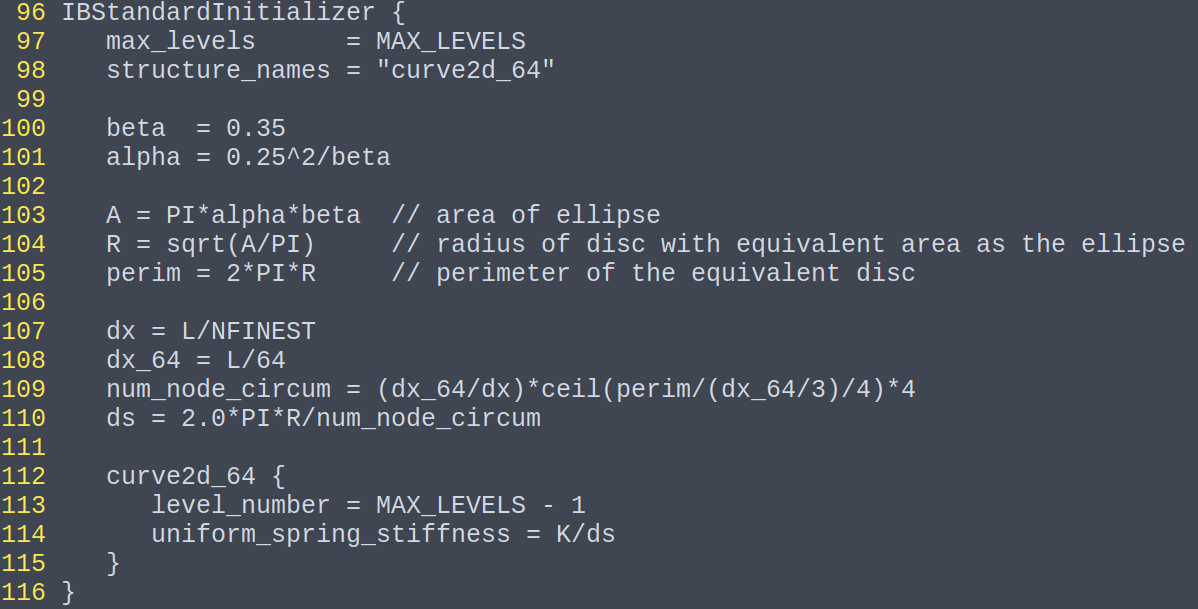
\includegraphics[width=0.5\textwidth]{Graphs/IB-ex1/input_IBStandardInitializer_initial.png}
\end{center}

The structure is named \verb|curve2d_64|, which points the program to open the files with that base name to initialize the structure. The structure lives on the level number \verb|MAX_LEVELS - 1|, which is the finest level number. The input file also specified a uniform spring stiffness of \verb|K/ds|, which overrides the value in the \verb|.spring| file.

We can run this example in the same way that we ran the Navier-Stokes example
\begin{verbatim}
./main2d input2d
\end{verbatim}
As before, we can open visit, click \verb|Open|, navigate to the example directory, and open the \verb|viz_IB2d| folder. In addition to the \verb|dumps.visit| file, which points to the Eulerian data, it also contains a \verb|lag_data.visit| file, which points to the Lagrangian data. 

\begin{center}
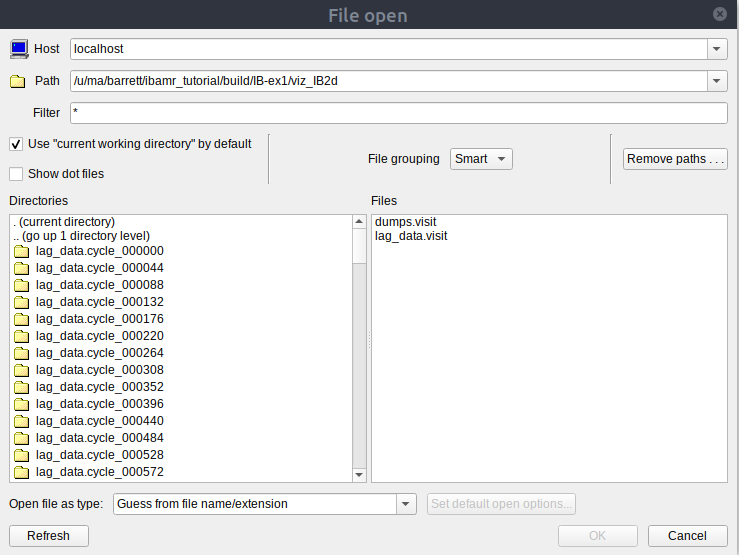
\includegraphics[width=0.5\textwidth]{Graphs/IB-ex1/visit_open_file.png}
\end{center}

Open the Lagrangian file, and add a plot of the mesh by selecting \verb|Add|, the \verb|Mesh|, the \verb|curve2d_64_mesh|. Make sure to press \verb|Draw| to make the plot appear in the window. To increase the width of the line, double click the \verb|curve2d_64_mesh| option to bring up the \verb|Mesh plot attributes| window. You can increase the line width, then apply the changes. Also open the \verb|dumps.visit| file, and add a pressure plot via the \verb|Pseudocolor| option. VisIt will ask if you want to create a database correlation. These are used to correlate two separate databases and use a single time slider to move advance both databases simultaneously. If opt not to create one, you can create one later through the \verb|Controls| and \verb|Database correlations| tab.

\begin{center}
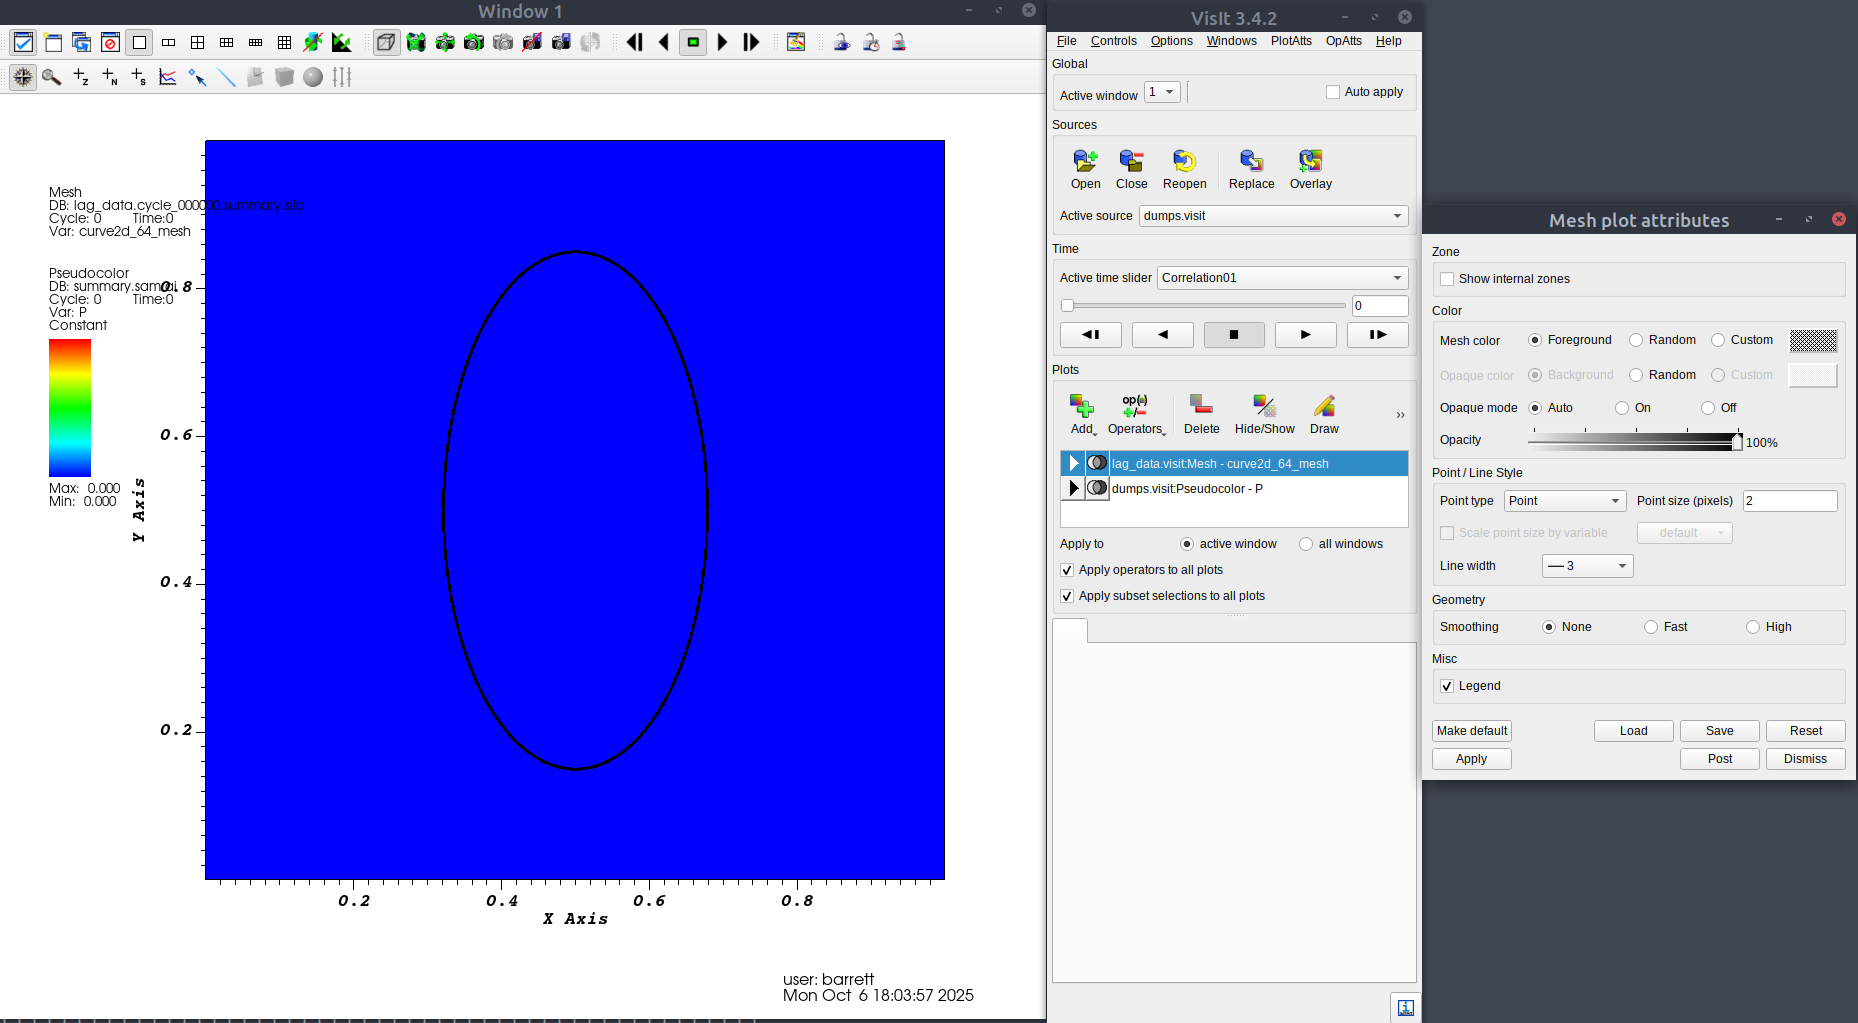
\includegraphics[width=0.9\textwidth]{Graphs/IB-ex1/initial_condition.png}
\end{center}

As before, you can step through time by pressing the play button.

Now we will add adaptive mesh refinement to this simulation. In the build directory, open the input file, and change \verb|MAX_LEVELS| from 1 to 2. This will add an additional level of refinement. Note the current refinement ratio is set to 4, so this additional level will have an equivalent uniform grid size of $N = 256$ points in each direction.

\begin{center}
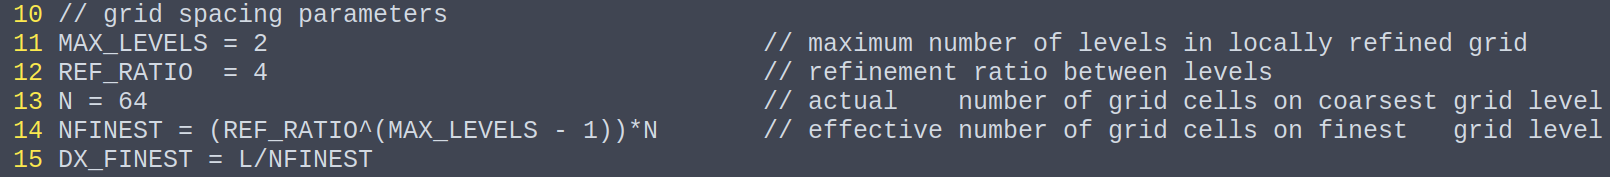
\includegraphics[width=0.9\textwidth]{Graphs/IB-ex1/max_refinement_2.png}
\end{center}

Before we run the simulation, we should make sure that the structure is refined as well. To do this, we need to point the \verb|IBStandardInitializer| database towards a different structure file, \verb|curve2d_256|. Note that all the constants computed in the database will automatically adjust for a change in grid spacing.

\begin{center}
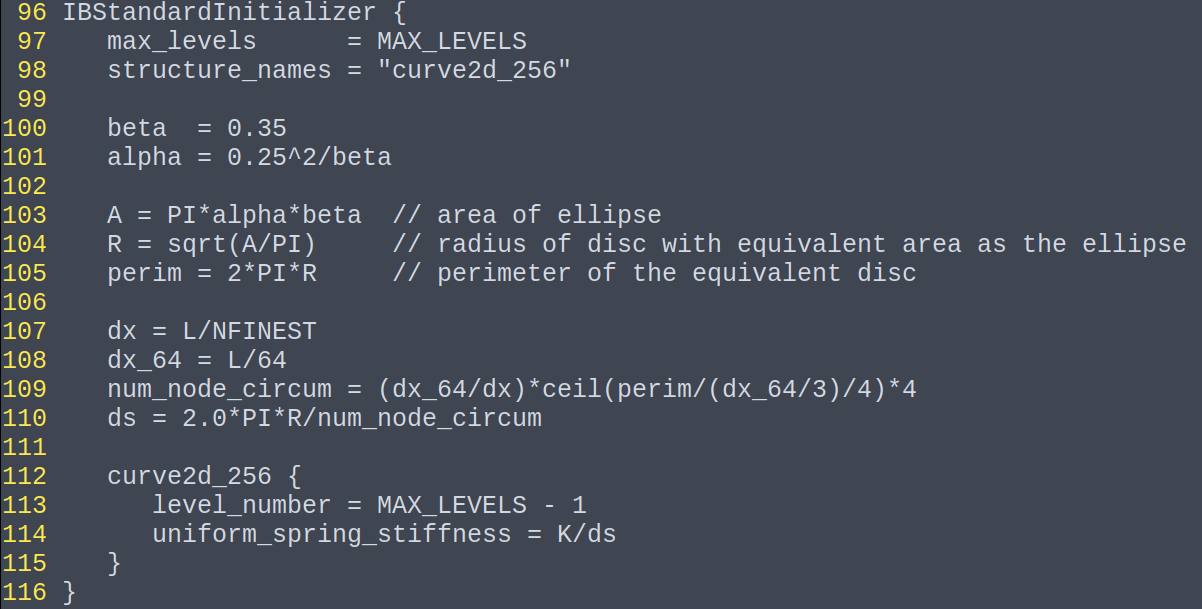
\includegraphics[width=0.5\textwidth]{Graphs/IB-ex1/IB_StandardInitiailzer_modified_input.png}
\end{center}

With the input file modified, we can rerun the example and open the visualization files as described above.

\subsection{IBAMR Major Concepts}
IBAMR borrows heavily from SAMRAI concepts, and in a lot of ways, is a application that lives on top of SAMRAI's data structures and algorithms.

The \verb|PatchHierarchy<NDIM>| object manages all Eulerian data and the layout of data on the adaptive grid. It is composed of sequences of \verb|PatchLevel<NDIM>| objects that are manage data for a specific grid spacing. Each \verb|PatchLevel<NDIM>| object contains a sequence of \verb|Patch<NDIM>| objects, each of which consists of a logically rectangular box of grid cells. Data on a patch is stored according to a patch data index, which is represented by an \verb|int|. Associated patch data can be accessed from by patch by the \verb|Patch<NDIM>| member function \verb|getPatchData()|. Note that patch data can correspond to cell, side, face, edge, or node centered dataa, and must be casted to the appropriate type before use. Typically, patch data indices are retrieved using the \verb|VariableDatabase<NDIM>| object, which will map pairs of \verb|Variable| and \verb|VariableContext| to patch data indices. The typical policy of IBAMR is for \verb|Variable| objects to correspond to specific state data, while \verb|VariableContext| objects correspond to time points. For example, the following code will retrieve the current velocity patch index from an \verb|INSStaggeredHierarchyIntegrator| object
\begin{verbatim}
auto var_db = VariableDatabase<NDIM>::getDatabase();
Pointer<SideVariable<NDIM, double>> u_var = ins_integrator->getVelocityVariable();
const int u_idx = var_db->mapVariableAndContextToIndex(u_var, ins_integrator->getCurrentContext());
\end{verbatim}
With that patch index, we can compute various quantities on the \verb|PatchHierarchy<NDIM>|. For example, we can compute the cell centered velocity magnitude by looping across all patches, interpolating velocities to cell centers, and computing the magnitude of the vector. The following code will do that.
\begin{verbatim}
Pointer<CellVariable<NDIM, double>> u_mag_var = new CellVariable<NDIM, double>("U_MAG");
auto var_db = VariableDatabase<NDIM>::getDatabase();
const int u_mag_idx = var_db->registerVariableAndContext(u_mag_var, var_db->getContext("CTX"));
for (int ln = 0; ln <= patch_hierarchy->getFinestLevelNumber(); ++ln)
{
  Pointer<PatchLevel<NDIM>> level = patch_hierarchy->getPatchLevel(ln);
  level->allocatePatchData(u_mag_idx);
  for (PatchLevel<NDIM>::Iterator p(level); p; p++)
  {
    Pointer<Patch<NDIM>> patch = level->getPatch(p());
    Pointer<CellData<NDIM, double>> u_mag_data = patch->getPatchData(u_mag_idx);
    Pointer<SideData<NDIM, double>> u_data = patch->getPatchData(u_idx);
    for (CellIterator<NDIM> ci(patch->getBox()); ci; ci++)
    {
      const CellIndex<NDIM>& idx = ci();
      double u_mag_sq = 0.0;
      for (int axis = 0; axis < NDIM; ++axis)
      {
        SideIndex<NDIM> up(idx, axis, 1), low(idx, axis, 0);
        double u = 0.5*((*u_data)(up) + (*u_data)(low));
        u_mag_sq += u * u;
      }
      (*u_mag_data)(idx) = std::sqrt(u_mag_sq);
    }
  }
}
\end{verbatim}
Note that we must allocate the patch data for \verb|u_mag_idx| before we can use it. Patch data stored with the \verb|getCurrentContext()| context is always allocated. The scratch and new context data may or may not be allocated. Efficient routines to compute various quantities can be found in the \verb|HierarchyMathOps| or \verb|HierarchyDataOpsReal| classes.

The major algorithms used in IBAMR are the \verb|HierarchyIntegrator| objects, which know how to integrate certain equations on a \verb|PatchHierarchy|. The main base integrators are
\begin{itemize}
\item \verb|AdvDiffHierarchyIntegrator| which can integrate advection diffusion reaction equations. It can be broken down further into two subclasses
\begin{itemize}
  \item \verb|AdvDiffSemiImplicitHierarchyIntegrator| uses a semi-implicit, method of lines approach to descritize equations.
  \item \verb|AdvDiffPredictorCorrectorHierarchyIntegrator| is an older integrator that does not see much use. I don't know what this does...
\end{itemize}
\item \verb|INSHierarchyIntegrator| which can integrate various forms of the Navier-Stokes equations. It has several subclasses
  \begin{itemize}
    \item \verb|INSStaggeredHierarchyIntegrator| is the standard Navier-Stokes integrator which uses a staggered discretization of the momentum equation, storing velocities as \verb|SideVariable<NDIM, double>| type and pressure as a \verb|CellVariable<NDIM, double>| type. This is the standard integrator that should be used in most applications.
    \item \verb|INSCollocatedHierarchyIntegrator| discretizes the momentum equation with a collocated discretization, storing velocities and pressures as \verb|CellVariable<NDIM, double>| types.
    \item \verb|INSVCStaggeredHierarchyIntegrator| discretizes the Navier-Stokes equations with spatially varying viscosity and density terms. Note that this utilizes the \verb|AdvDiffHierarchyIntegrator| class to advect the viscosity and density. This class further breaks down into non-conservative and conservative discretizations.
  \end{itemize}
\item \verb|IBHierarchyIntegrator| which can integrator the immersed boundary equations. Currently, the only concrete implementation is the \verb|IBExplicitHierarchyIntegrator| class, which treats the immersed boundary explicitly in time.
\end{itemize}

To complement the integrators and provide a method to customize the equations, each integrator can handle specialized source terms, forcing functions, or strategy classes. Below covers some of the typicaly use cases for each of these integrator classes.

\subsubsection{AdvDiffHierarchyIntegrator}
Advected variables can be registered with the \verb|AdvDiffHierarchyIntegrator| object to be integrated in the order in which they are registered. The advection diffusion integrators provide frameworks to set convective discretizations, variable diffusion coefficients, and source terms. For example, in \verb|navier_stokes-ex5|, a temperature proxy variable used in the Boussinesq approximation is registered in the source code \verb|example.cpp|: \\
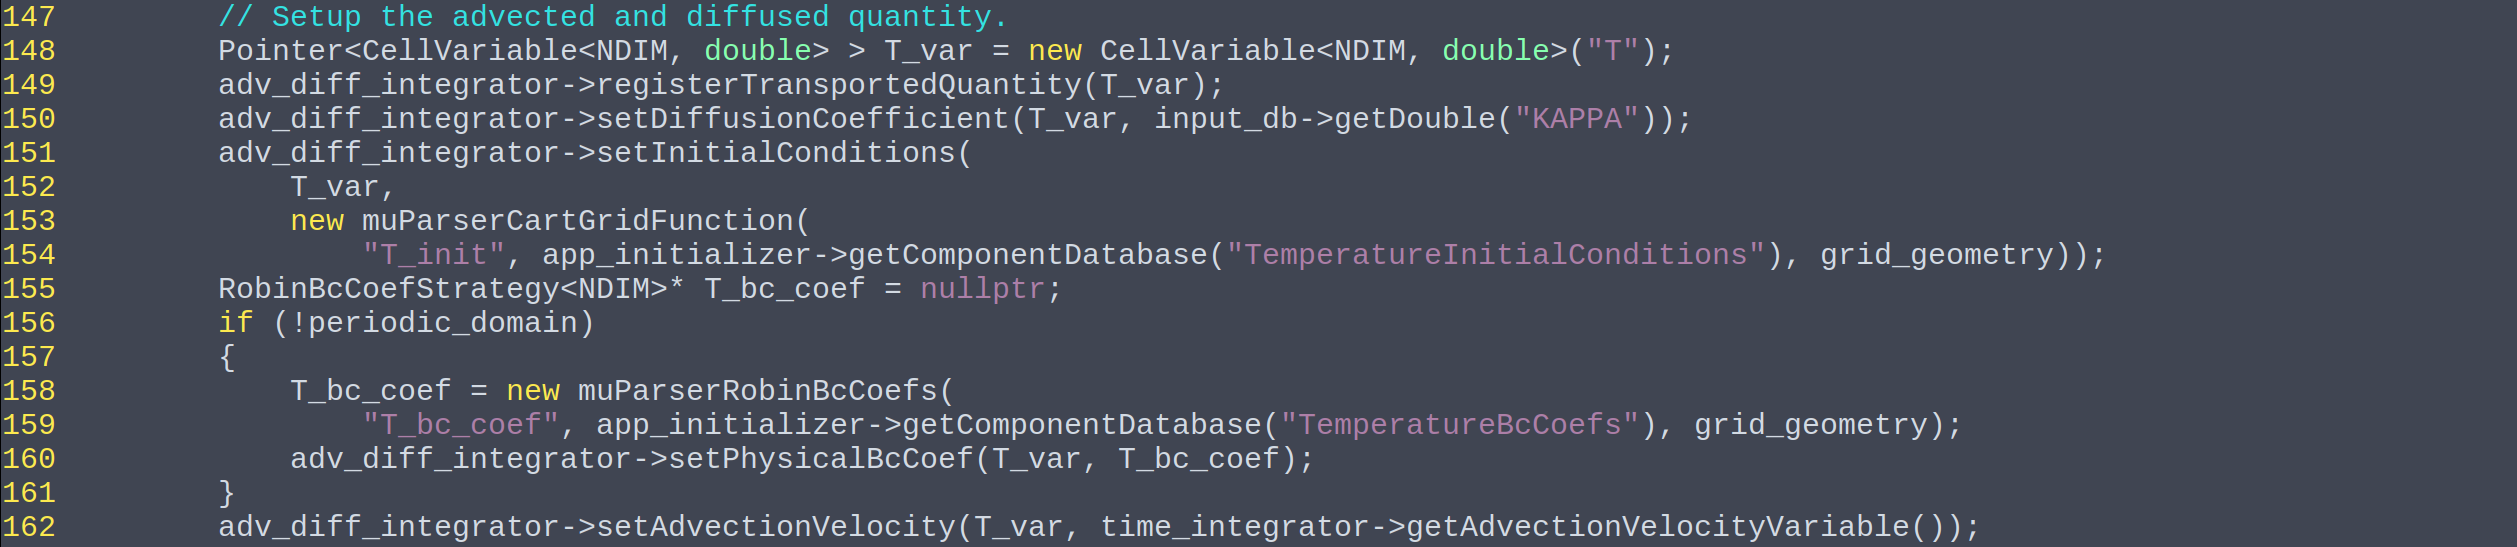
\includegraphics[width=\textwidth]{Graphs/NS-ex5/advected_quantity.png}


\paragraph{Convective Operators:} The convective discretization is typically set in the input file. For example, in \verb|navier_stokes-ex5|, the input file has the following set of options \\
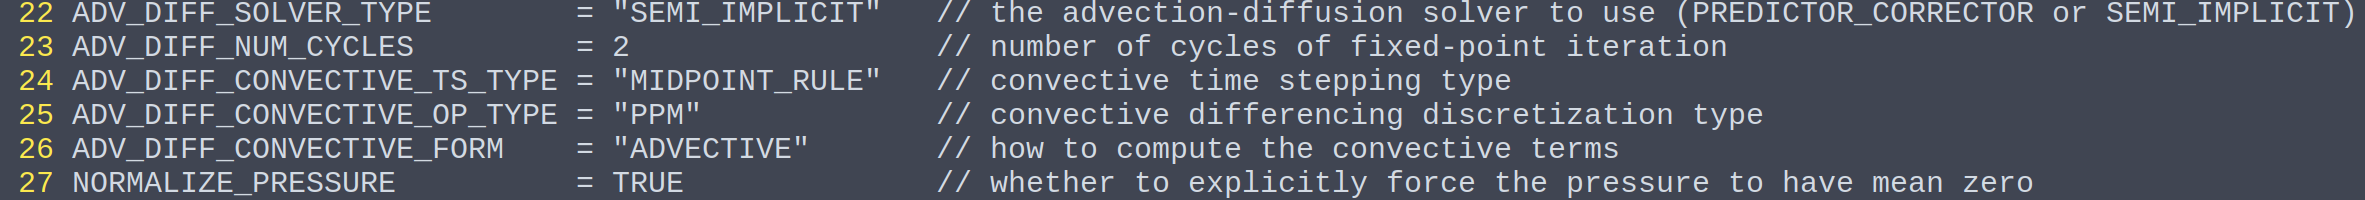
\includegraphics[width=\textwidth]{Graphs/NS-ex5/AdvDiffIntegrator_options.png} 
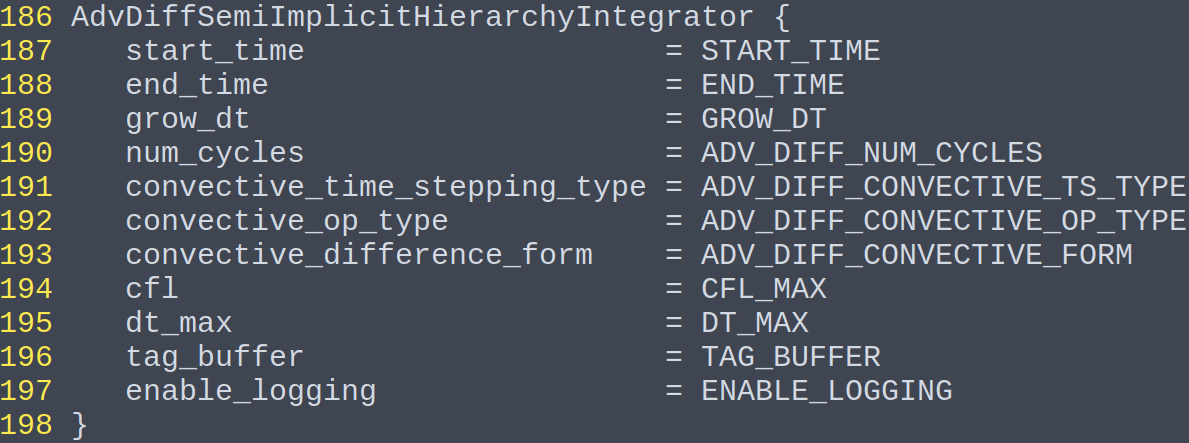
\includegraphics[width=0.52\textwidth]{Graphs/NS-ex5/AdvDiffIntegrator_DB.png}

In this case, the input file sets the convective operator to use the \verb|PPM| operator, discretized in \verb|ADVECTIVE_FORM|, using a \verb|MIDPOINT_RULE| to discretize in time.

IBAMR has several default convective operators to choose from:
\begin{itemize}
\item \verb|PPM| uses a piecewise parabolic method,
\item \verb|CUI| uses a cubic upwinded interpolant method,
\item \verb|WAVE_PROP| uses a wave propagation method,
\item \verb|CENTERED| uses centered differences.
\end{itemize}
The convective terms can be integrated using \verb|MIDPOINT_RULE|, \verb|TRAPEZOIDAL_RULE|, or \verb|FORWARD_EULER|. Note that \verb|TRAPEZOIDAL_RULE| is an explicit RK2 method. Each convective operator can discretize the equations in either \verb|ADVECTIVE| form: $\bu\cdot\grad Q$ or \verb|CONSERVATIVE| form: $\grad\cdot(\bu Q)$.

\paragraph{Diffusion Coefficients:}
Uniform diffusion coefficients can be set by the call \verb|setDiffusionCoefficient| in the \verb|AdvDiffHierarchyIntegrator| object. If no diffusion coefficient is used, or the diffusion coefficient is \emph{exactly} equal to 0.0, no diffusion solver will be used. Otherwise, a Krylov solver will be used to solve the resulting implicit system, depending on the time stepping type specified.

Variable diffusion coefficients can be set by registering a variable diffusion coefficient with the \verb|AdvDiffHierarchyIntegrator| object via the call \verb|registerDiffusionCoefficientVariable|. Note that the variable registered must be of type \verb|SideVariable<NDIM, double>|. Then, a function that specifies the value of the diffusion coefficient should be registered, followed by setting the diffusion variable of the appropriate diffused quantities. For example, assuming \verb|DiffusionCoefficient| is a class that extends \verb|CartGridFunction|, the following code will set a variable coefficient for the advected quantity \verb|Q_var|.
\begin{verbatim}
Pointer<SideVariable<NDIM, double>> D_var = new SideVariable<NDIM, double>("D");
adv_diff_integrator->registerDiffusionCoefficientVariable(D_var);
Pointer<CartGridFunction> D_fcn = new DiffusionCoefficient();
adv_diff_integrator->setDiffusionCoefficientFunction(D_var, D_fcn);
adv_diff_integrator->setDiffusionCoefficientVariable(Q_var, D_var);
\end{verbatim}

\paragraph{Source Terms:}
Source terms in the advection diffusion integrator can be set in a similar method. A \verb|CellVariable<NDIM, double>| object must be registered with the integrator. Then, the function that specifies the source must be registered and the source term must be set for the advected variable. If \verb|SourceFunction| is a class that extends \verb|CartGridFunction|, the following code will set a source term for the advected quantity \verb|Q_var|.
\begin{verbatim}
Pointer<CellVariable<NDIM, double>> R_var = new CellVariable<NDIM, double>("R");
adv_diff_integrator->registerSourceTerm(R_var);
Pointer<CartGridFunction> R_fcn = new SourceFunction();
adv_diff_integrator->setSourceTermFunction(R_var, R_fcn);
adv_diff_integrator->setSourceTerm(Q_var, R_var);
\end{verbatim}

\subsubsection{INSStaggeredHierarchyIntegrator}
The \verb|INSHierarchyIntegrator| class and derived classes generally know how to solve the Navier-Stokes equations with different data centerings or variable coefficients. Our focus here is on the \verb|INSStaggeredHierarchyIntegrator| class, although the other classes function similarly. The \verb|INSStaggeredHierarchyIntegrator| class discretizes the constant coefficient Navier-Stokes equations on a staggerd grid, with the velocity stored as type \verb|SideVariable<NDIM, double>| and pressure as type \verb|CellVariable<NDIM, double>|. These integrator classes allow for a substantial amount of customization.

\paragraph{Forcing Functions:}
The computation of the body force must be done in an extension of the \verb|CartGridFunction| interface. Note the force must be evaluated in accordance with the grid spacing used for the velocity. For example, if the integrator is of type \verb|INSStaggeredHierarchyIntegrator|, the data index provided to the forcing function corresponds to type \verb|SideData<NDIM, double>|. The forcing function can be registered with the \verb|INSHierarchyIntegrator| with the call \verb|registerBodyForceFunction|. 

\paragraph{Viscoelasticity:}
Viscoelastic fluids that follow a Maxwell type model can be added via the \verb|CFINSForcing| class. It requires a derived class of type \verb|CFStrategy| be written that can compute the right hand side of the upper convective derivative and the transformation from the advected tensor to the stress tensor. Classes for Oldroyd-B, Giesekus, and Rolie-Poly already exist in IBAMR, and can be specified by the \verb|fluid_model| parameter in the input database.

The class \verb|CFINSForcing| is a specific implementation of a \verb|CartGridFunction| whose application of \verb|setDataOnPatchHierarchy| computes the divergence of the extra stress tensor. Therefore, to add viscoelasticity to a fluid solver, one needs to register the \verb|CFINSForcing| object with the \verb|INSHierarchyIntegrator| via the \verb|registerBodyForceFunction| function.

\paragraph{Boundary Conditions:}
Boundary conditions can be registered with the Navier-Stokes integrator. Typically, boundary conditions will be read from the input file by the class \verb|muParserRobinBcCoef|, which can parse strings into mathematical functions. The input file for these conditions specify the $a$, $b$, and $g$ coefficients on each box face, for each spatial dimension. Boundary conditions take the form of $ a\bu + b\bbtau\cdot\bn = \bg$, in which $\bbtau = -p\bbI + \frac{\mu}{2}\parens{\grad\bu + \grad\bu^\text{T}}$ is the Newtonian stress and $\mu$ is the fluid viscosity. Current implementations require that at any physical location, the values of $a$ and $b$ satisfy that either $a = 1$ or $b = 1$ and that $a + b = 1$.

In all cases, periodic boundaries take prescendence over physical boundary conditions. Periodic conditions are specified in the \verb|CartesianGeometry| database in the input file.

A typical implementation would look like this
\begin{verbatim}
vector<RobinBcCoefStrategy<NDIM>*> u_bc_coefs(NDIM, nullptr);
for (unsigned int d = 0; d < NDIM; ++d)
  {
  const std::string bc_coefs_name = "u_bc_coefs_" + std::to_string(d);
  const std::string bc_coefs_db_name = "VelocityBcCoefs_" + std::to_string(d);
  u_bc_coefs[d] = new muParserRobinBcCoefs(
    bc_coefs_name, app_initializer->getComponentDatabase(bc_coefs_db_name), grid_geometry);
  }
time_integrator->registerPhysicalBoundaryConditions(u_bc_coefs);
\end{verbatim}
and the corresponding input file would look like
\begin{verbatim}
VelocityBcCoefs_0 {
   acoef_function_0 = "1.0"
   acoef_function_1 = "1.0"
   acoef_function_2 = "1.0"
   acoef_function_3 = "1.0"

   bcoef_function_0 = "0.0"
   bcoef_function_1 = "0.0"
   bcoef_function_2 = "0.0"
   bcoef_function_3 = "0.0"

   gcoef_function_0 = "0.0"
   gcoef_function_1 = "0.0"
   gcoef_function_2 = "0.0"
   gcoef_function_3 = "0.0"
}
\end{verbatim}
with another database for \verb|VelocityBcCoefs_1|. This boundary condition sets up no slip for the horizontal component of the velocity.

\subsubsection{IBHierarchyIntegrator}
\paragraph{IBStrategy:}

\paragraph{IBMethod:}

\paragraph{IBFEMethod:}

\section{Navier Stokes Ex 5}
The example \verb|navier_stokes-ex5| models stratefied layer of fluids marked by temperature differences. The Boussinesq approximation is used to compute the force of gravity on the system. The temperature of the fluid is modeled by an advection-diffusion equation
\begin{equation}\label{eq:T}
\frac{\partial T}{\partial t} + \bu\cdot\grad T = D\Lap T,
\end{equation}
and an extra force is added to the momentum equation
\begin{equation}\label{eq:F}
\bF = \gamma\bg\parens{T - T_0},
\end{equation}
in which $T_0$ is the baseline temperature and $\bg$ is the force of gravity, here assumed to orient in the negative $y$ direction.

As before, we can navigate to the build directory and build the example
\begin{verbatim}
cd ibamr_tutorials/build && make -j4 examples
cd navier_stokes-ex1
./main2d input2d
\end{verbatim}
If we look at the source code, we can see the \verb|BoussinesqForcing| source and header files as well as the main source \verb|example.cpp|. The main source code contains very similar code to that of \verb|navier-stokes_ex1|, with the addition of the \verb|AdvDiffHierarchyIntegrator| class that is registered with the fluid solver. This new integrator will integrate the temperature in equation \eqref{eq:T}.
\begin{center}
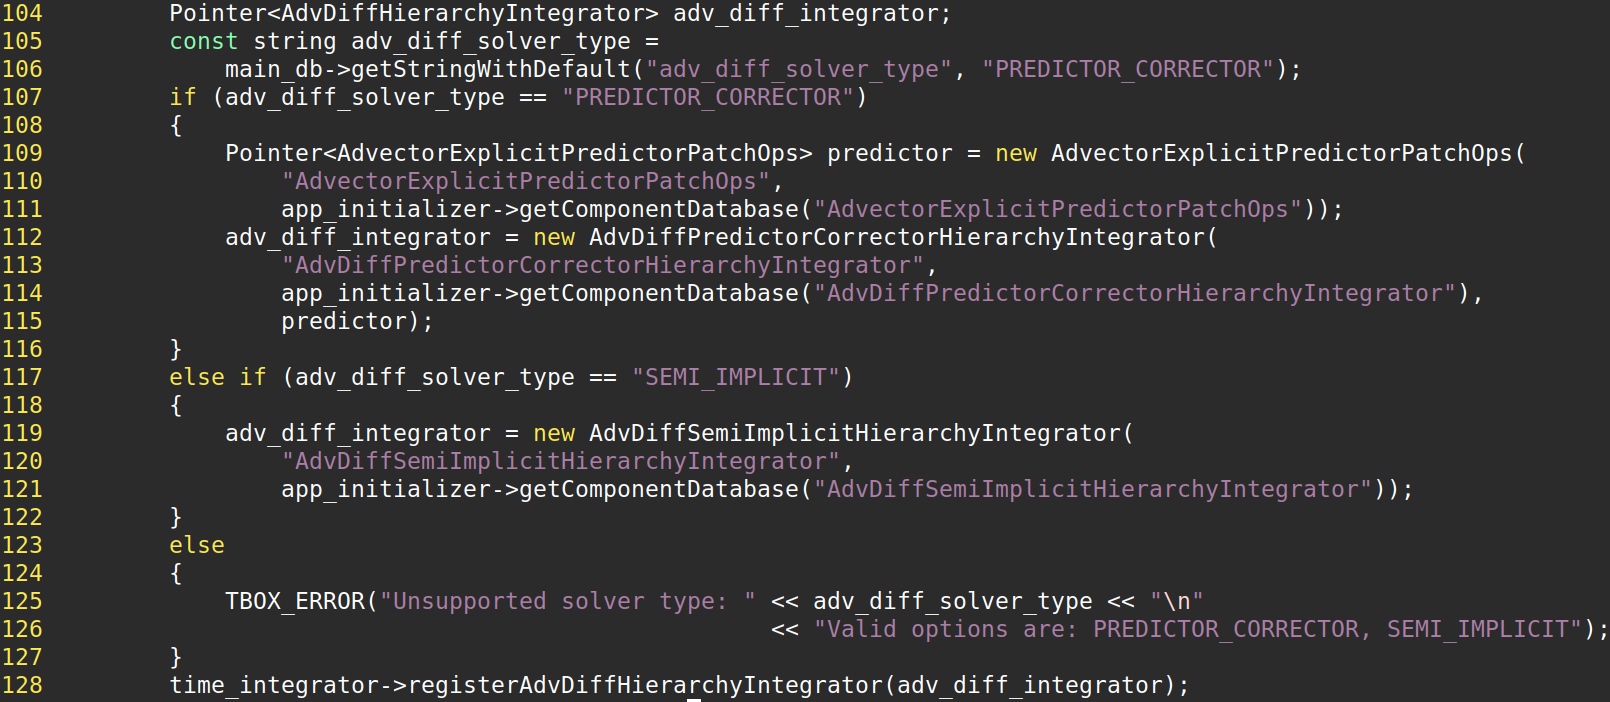
\includegraphics[width=0.8\textwidth]{Graphs/NS-ex5/source_AdvDiffIntegrator.png}
\end{center}

As noted earlier, the variable denoting the temperature $T$ is created and registered with the advection diffusion integrator.
\begin{center}
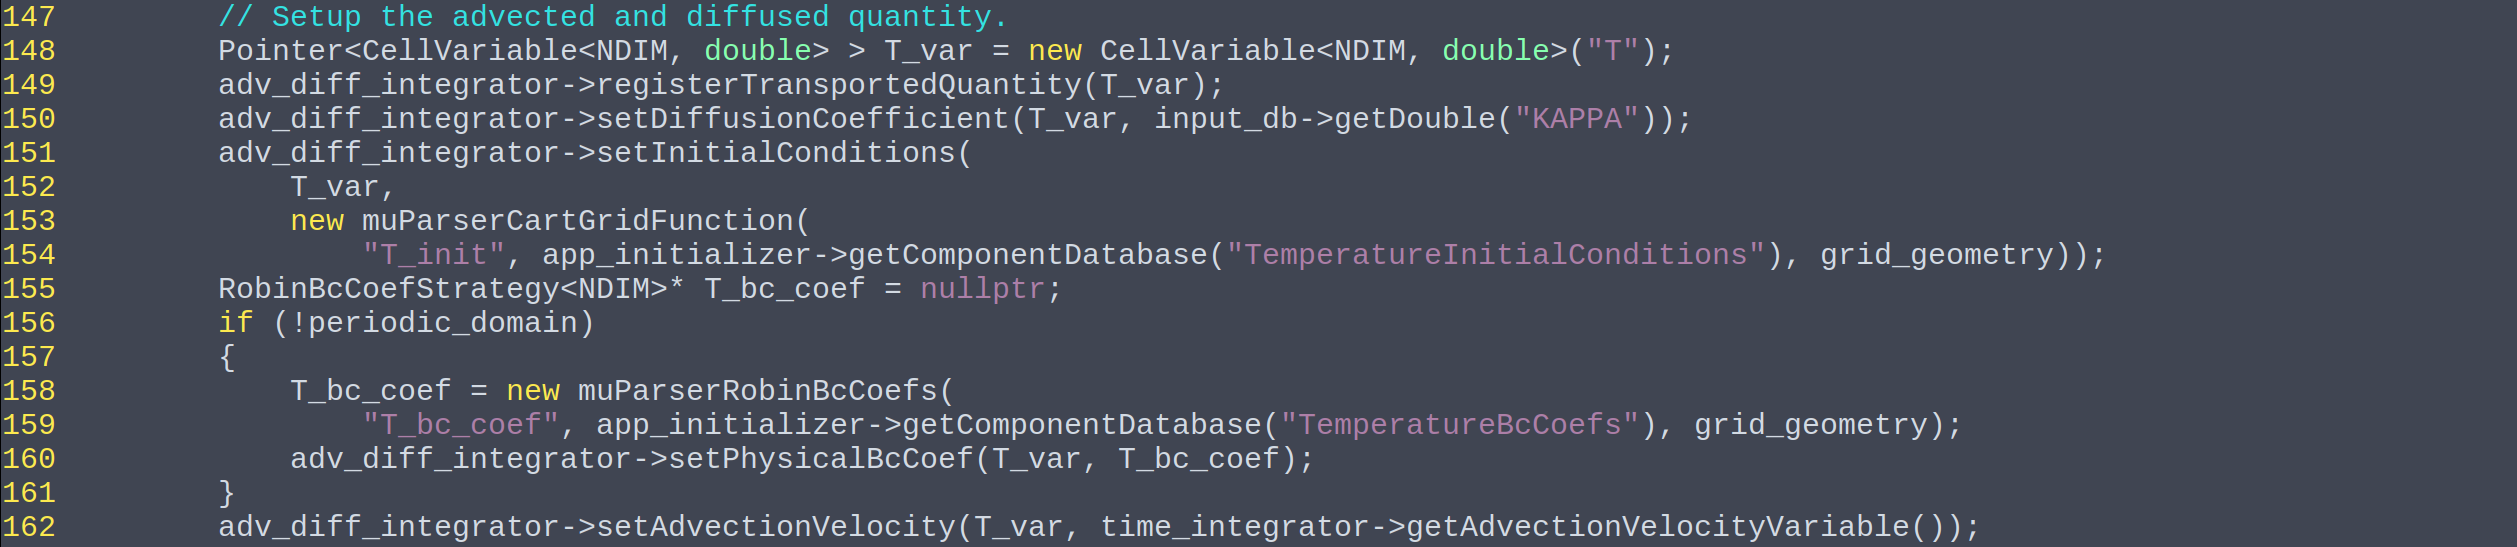
\includegraphics[width=\textwidth]{Graphs/NS-ex5/advected_quantity.png}
\end{center}

Finally, a \verb|BoussinesqForcing| object is registered with the integrator
\begin{center}
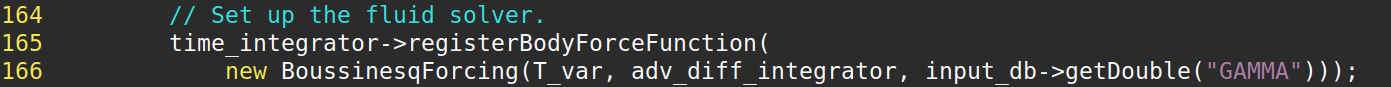
\includegraphics[width=0.8\textwidth]{Graphs/NS-ex5/source_registerForce.png}
\end{center}

As noted in the section on forces for the Navier-Stokes integrators, the class \verb|BoussinesqForcing| is an extension of a \verb|CartGridFunction| that can evaluate equation \eqref{eq:F} on the patch hierarchy. On creation, it takes the variable representing the temperature, the advection diffusion integrator that manages the data, and the parameter $\gamma$, as seen in the header file
\begin{center}
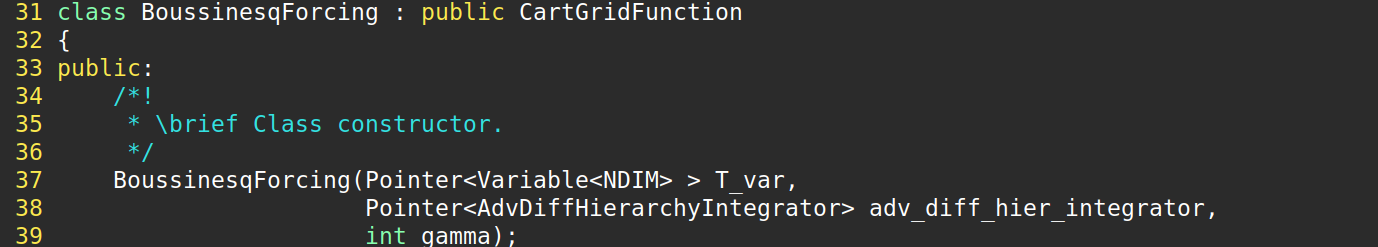
\includegraphics[width=0.8\textwidth]{Graphs/NS-ex5/Boussinesq_header_constructor.png}
\end{center}
The corresponding source file \verb|BoussinesqForcing.cpp| contains two important functions, \verb|setDataOnPatchHierarchy| and \verb|setDataOnPatch|.

In order to evaluate the force in equation \eqref{eq:F} on cell sides, we must interpolate the cell centered data to the side of a cell, then multiple by $-\gamma$. To do the interpolation, we require one layer of ghost cells to be filled in. The function \verb|setDataOnPatchHierarchy| allocates scratch data for \verb|T_var| (if necessary), then fills in ghost cells using the class \verb|HierarchyGhostCellInterpolation|, which contains general routines to make filling ghost cells easy. Then the function loops over levels and calls \verb|setDataOnPatchLevel|, which by default will loop over patches and call \verb|setDataOnPatch|.

The actual computation of the force is done in \verb|setDataOnPatch|. First, the cell data corresponding to the scratch context is retrieved from the patch. Then, we loop over all cell sides whose normal points in the $y$ direction. We interpolate the cell data to the cell side using simple averaging, and evaluate the force.
\begin{center}
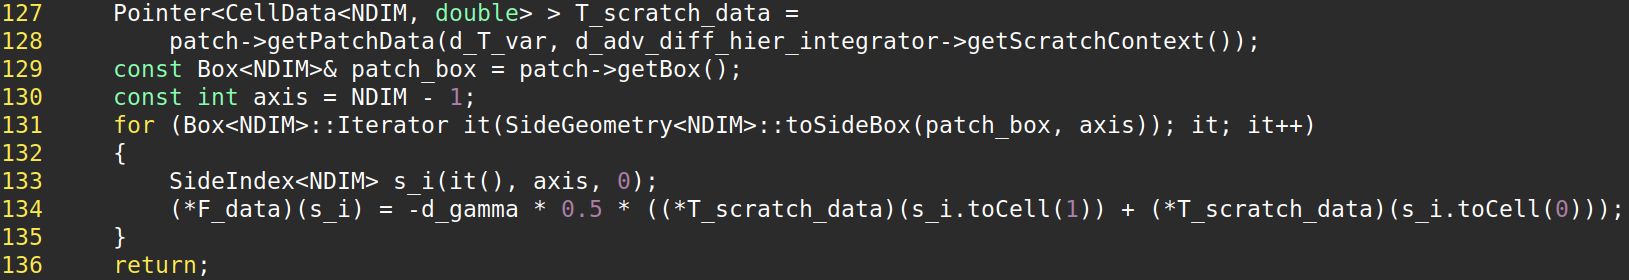
\includegraphics[width=0.8\textwidth]{Graphs/NS-ex5/Boussinesq_setDataOnPatch.png}
\end{center}

\subsection{Adding a Simple Reaction System}
We can add a simple reaction system to this model by adding two new advected variables $R$ and $Q$. Let's say the reaction system will be
\begin{align}
\frac{\partial Q}{\partial t} + \bu\cdot\grad Q &= D_Q \Lap Q - \kappa Q(1 - R), \label{eq:Q}\\
\frac{\partial R}{\partial t} + \bu\cdot\grad R &= D_R \Lap R + \kappa Q(1 - R). \label{eq:R}
\end{align}
To accomplish this, we need to add two advected quantities, $Q$ and $R$, and write two source functions \verb|QSourceFunction| and \verb|RSourceFunction|. To start, we can checkout the branch that adds a skeleton for these functions.
\begin{verbatim}
cd ibamr_tutorial/ibamr_tutorial
git pull && git checkout add_source
\end{verbatim}
In the source directory \verb|navier_stokes-ex5|, there should now be two additional files \verb|QSourceFunction.h| and \verb|QSourceFunction.cpp|. To complete the \verb|QSourceFunction| class, we need to be able to evaluate the source term in equation \eqref{eq:Q}. To evaluate this term, we need the values of $\kappa$, $Q$, and $R$. Therefore, we will need to store the patch data corresponding to $Q$ and $R$ and have a \verb|double| that corresponds to the value of $\kappa$. These will be stored as member variables of the class. We also need to update the constructor to ensure these objects are avaiable upon construction of the object
\begin{center}
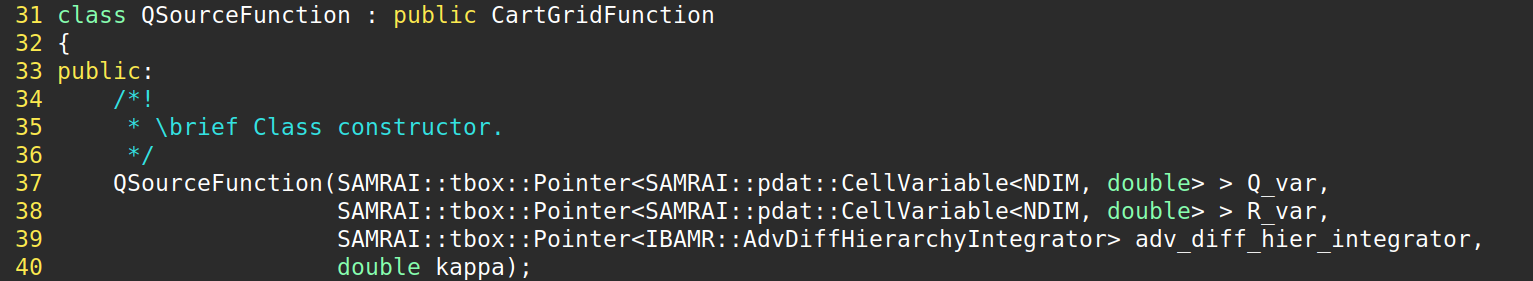
\includegraphics[width=0.8\textwidth]{Graphs/NS-ex5/add_src/header_update_constructor.png} \\
\vspace{0.5em}
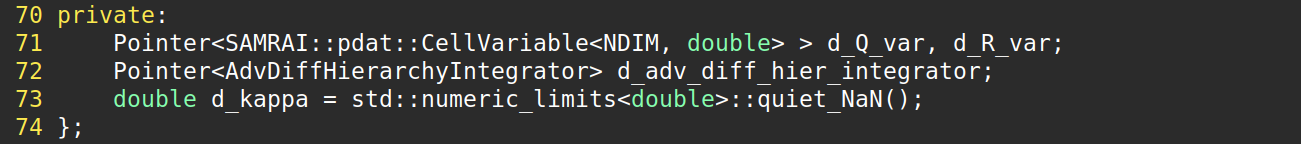
\includegraphics[width=0.8\textwidth]{Graphs/NS-ex5/add_src/header_update_member_vars.png}
\end{center}

In the implementation file, we need to update the constructor to set the appropriate member variables. We also need to update the \verb|setDataOnPatch| function to correctly evaluate the source function. Note we do not need ghost cell information to evaluate this function. Therefore, the code that filled ghost cells in \verb|BoussinesqForcing| is not needed here.
\begin{center}
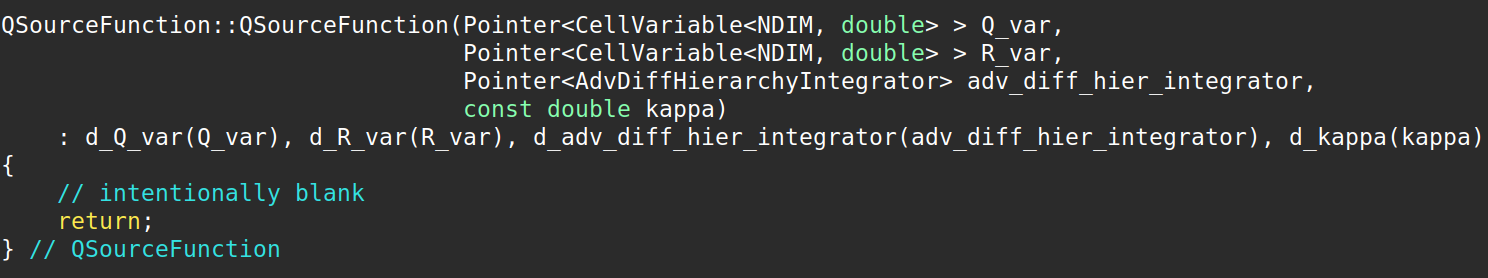
\includegraphics[width=0.8\textwidth]{Graphs/NS-ex5/add_src/source_constructor.png} \\
\vspace{0.5em}
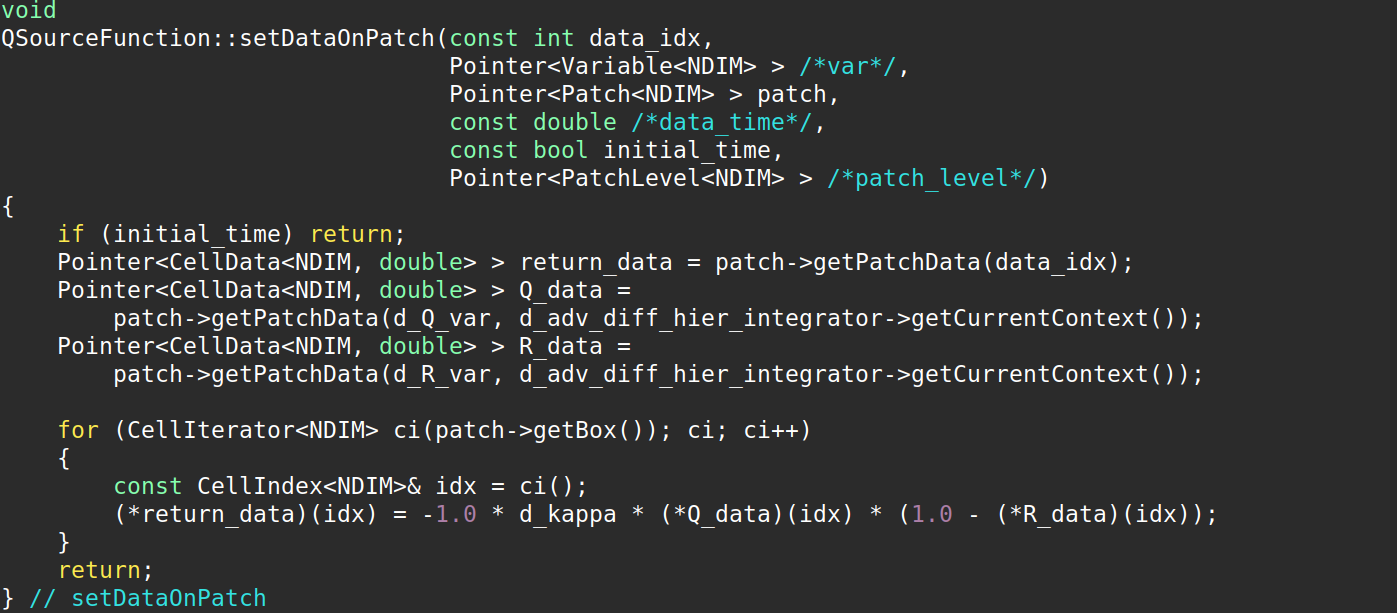
\includegraphics[width=0.8\textwidth]{Graphs/NS-ex5/add_src/source_setDataOnPatch.png}
\end{center}

We need to do the same for the class \verb|RSourceFunction|. Because the function for $R$ is the negative of the function for $Q$, we can simply copy the $Q$ files.
\begin{verbatim}
cp QSourceFunction.cpp RSourceFunction.cpp
cp QSourceFunction.h RSourceFunction.h
\end{verbatim}
You will need to make sure the names inside the source and header files are changed to their appropriate class, as well as fixing the sign of the operator. We also need to update the \verb|CMakeLists.txt| to ensure that the files are compiled.
\begin{center}
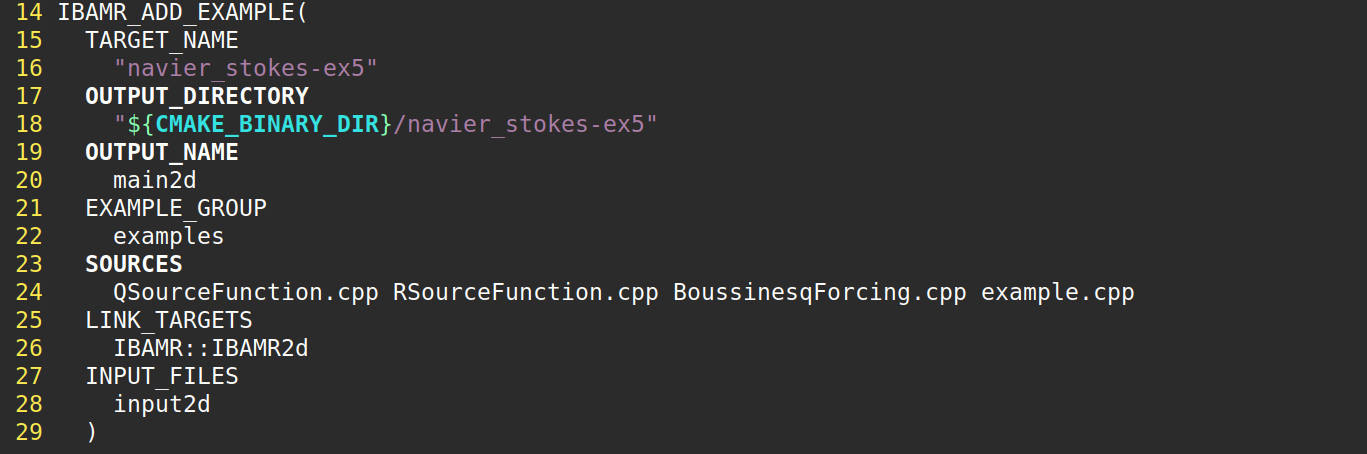
\includegraphics[width=0.8\textwidth]{Graphs/NS-ex5/add_src/cmake_lists.png}
\end{center}

Finally, we need to update the main driver to create and register two cell centered variables with the advection diffusion integrator. First, we add the header files to the main routine.
\begin{center}
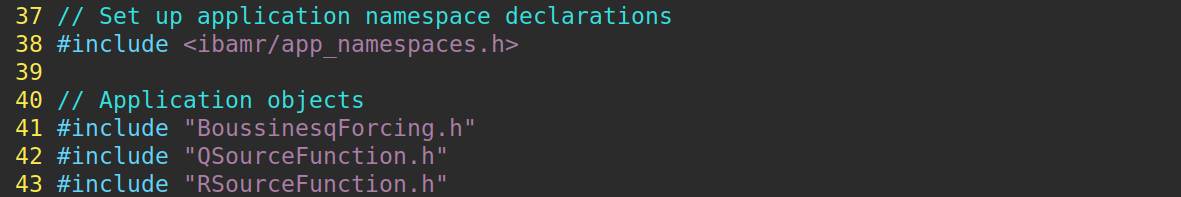
\includegraphics[width=0.8\textwidth]{Graphs/NS-ex5/add_src/main_add_headers.png}
\end{center}

Next, we create cell variables corresponding to $Q$ and $R$. We need to register them with the advection-diffusion solver as well as set coefficients, set advection velocities, and specify boundary and initial conditions. By default, initial conditions are set to 0 and boundary conditions default to linear extrapolation from interior values.

Finally, we need to create source variables that correspond to the sources for $Q$ and $R$. We register these with the advection-diffusion integrator, as well as register functions that set the source terms. As shown below, when we create the source functions, the rate constant is being read from the input file.

\begin{center}
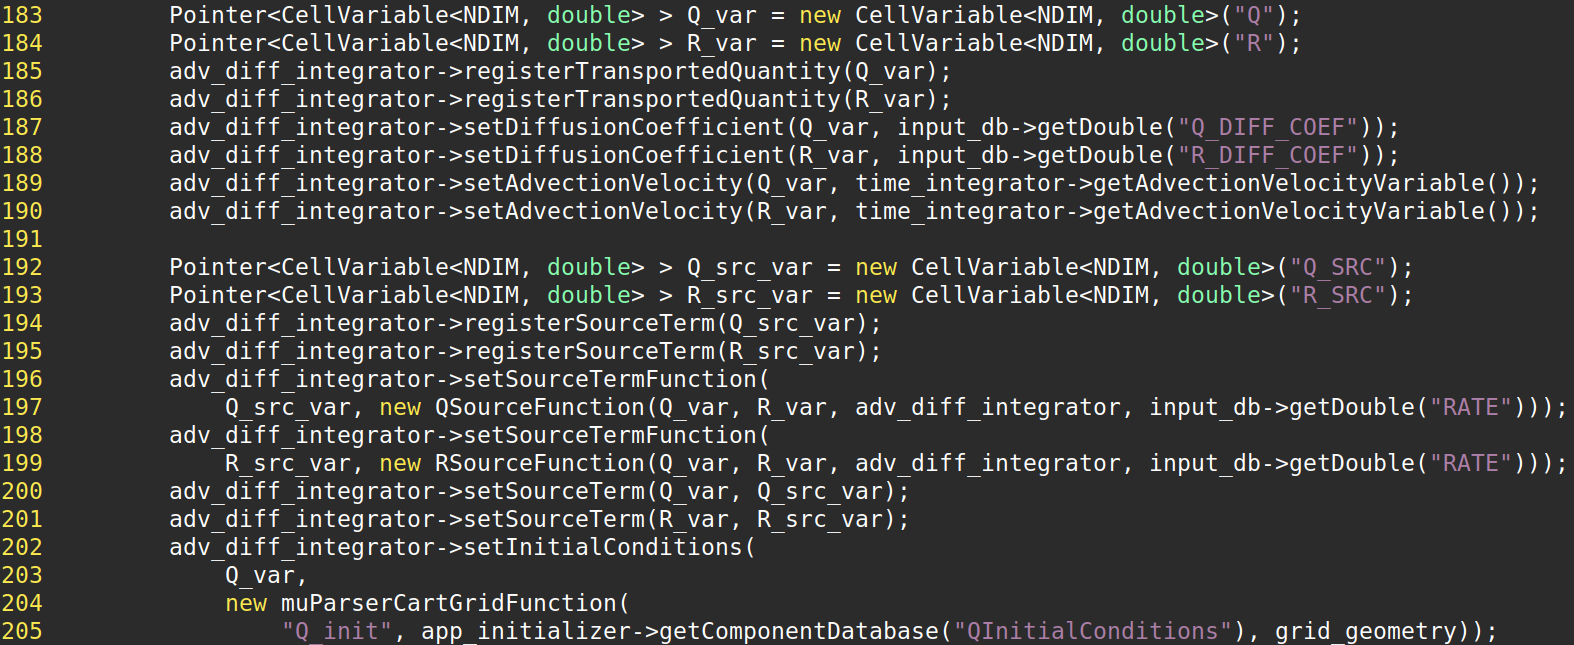
\includegraphics[width=0.8\textwidth]{Graphs/NS-ex5/add_src/main_add_sources.png}
\end{center}

With this, we can compile and run the new example as before. Make sure you edit the input file to specify the rate parameter \verb|RATE| and the diffusion coefficients \verb|Q_DIFF_COEF| and \verb|R_DIFF_COEF|.
\begin{verbatim}
cd ibamr_tutorials/build && make -j4 examples
cd navier_stokes-ex5
./main2d input2d
\end{verbatim}
\end{document}